\PassOptionsToPackage{table}{xcolor}
\documentclass[10pt]{beamer}
\usepackage[english]{babel}

\usetheme{metropolis}
\usepackage{smartdiagram}
\usepackage{listings}
\usepackage{booktabs}
\usepackage[scale=2]{ccicons}%creative commons
\setbeamercovered{transparent}%invisible by default
\usepackage{array}
\newcolumntype{L}[1]{>{\raggedright\let\newline\\\arraybackslash\hspace{0pt}}m{#1}}
\newcolumntype{C}[1]{>{\centering\let\newline\\\arraybackslash\hspace{0pt}}m{#1}}
\newcolumntype{R}[1]{>{\raggedleft\let\newline\\\arraybackslash\hspace{0pt}}m{#1}}

\usepackage{pgfplots}
\usepgfplotslibrary{dateplot}
\usepackage{tikz}
\usepackage{tikz-uml}
\usetikzlibrary{positioning,chains,fit,shapes,calc,automata,positioning}
\newcommand{\mycomment}[1]{}
\usepackage{fancyvrb}
\usepackage{ifpdf}                        % To check if pdflatex is used.

\ifpdf
  \DeclareGraphicsRule{*}{mps}{*}{}       % To include metapost files.
\fi
% *****************************************************************************
% Matematica 
% *****************************************************************************

%\usepackage{amssymb}
%\usepackage{mathtools}                    % Add support for cramped,
					  
%\usepackage[euler]{flexisym}
%\usepackage{breqn}                        % Breqn
%\makeatletter
%   \def\eqnumsize{\normalfont \Tf@font}      % Add support to Minion Pro
%\makeatother
%\setkeys{breqn}{labelprefix={eq:}}


%\usepackage{asymptote}
%\usepackage[loop, controls]{animate}

\graphicspath{{./}, {./Images/}}

\lstdefinelanguage{Kotlin}{
  keywords={package, as, typealias, this, super, val, var, fun, for, null, true, false, is, in, throw, return, break, continue, object, if, try, else, while, do, when, yield, typeof, yield, typeof, class, interface, enum, object, override, public, private, get, set, import, abstract, },
  keywordstyle=\color{blue}\bfseries,
  ndkeywords={@Deprecated, Int, Integer, Float, Double, String, Runnable, dynamic},
  ndkeywordstyle=\color{red}\bfseries,
  emph={println, return@, forEach,},
  emphstyle={\color{red}},
  identifierstyle=\color{black},
  sensitive=true,
  commentstyle=\color{gray}\ttfamily,
  comment=[l]{//},
  morecomment=[s]{/*}{*/},
  stringstyle=\color{gray}\ttfamily,
  morestring=[b]",
  morestring=[s]{"""*}{*"""},
}

\providecommand{\ie}{i.\,e.}
\providecommand{\Ie}{I.\,e.}
\providecommand{\eg}{e.\,g.}
\providecommand{\Eg}{E.\,g.} 

\metroset{block=fill}
\metroset{titleformat frame=smallcaps}

\title{Having fun with Kotlin coroutines}
%\subtitle{Ariadne's thread in Kotlin models of concurrency}
\subtitle{A first tour of concurrency models in Kotlin}

\date{\today}
\author[A. Candolini]{Alessandro Candolini}
%\institute{Department of Physics, University of Trieste}
% \titlegraphic{\hfill\includegraphics[height=1.5cm]{logo/logo}}

\begin{document}

\maketitle

\begin{frame}{Agenda}
  \setbeamertemplate{section in toc}[sections numbered]
  \tableofcontents[hideallsubsections]
\end{frame}

\section{We live in a concurrent world}
\begin{frame}[fragile]
	\begin{figure}
		\centering
		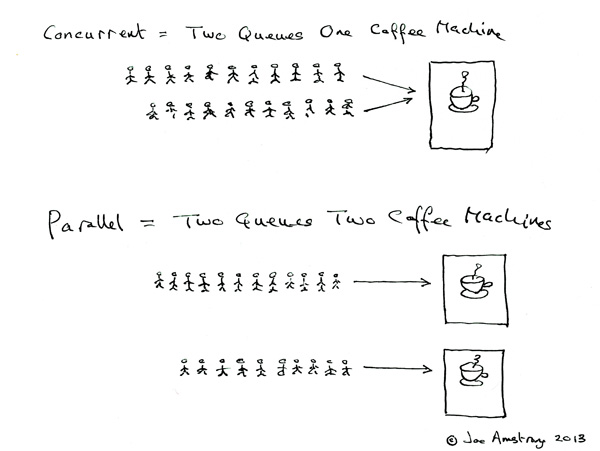
\includegraphics[width=.8\textwidth]{concurrency_coffee}
		\caption{\url{https://joearms.github.io/published/2013-04-05-concurrent-and-parallel-programming.html}}
	\end{figure}
\end{frame}
\begin{frame}[fragile]
Is concurrency relevant for mobile development?
	\begin{itemize} 
		\item<2-> IO (\eg, network, etc) 
		\item<3-> sensors (\eg, gps, etc) 
		\item<4-> UI events 
		\item<5-> platform lifecycle 
	\end{itemize}
\end{frame}
\begin{frame}[fragile]
\begin{columns}
\begin{column}{0.4\textwidth}
	\begin{center}
	\begin{figure}
		\centering
		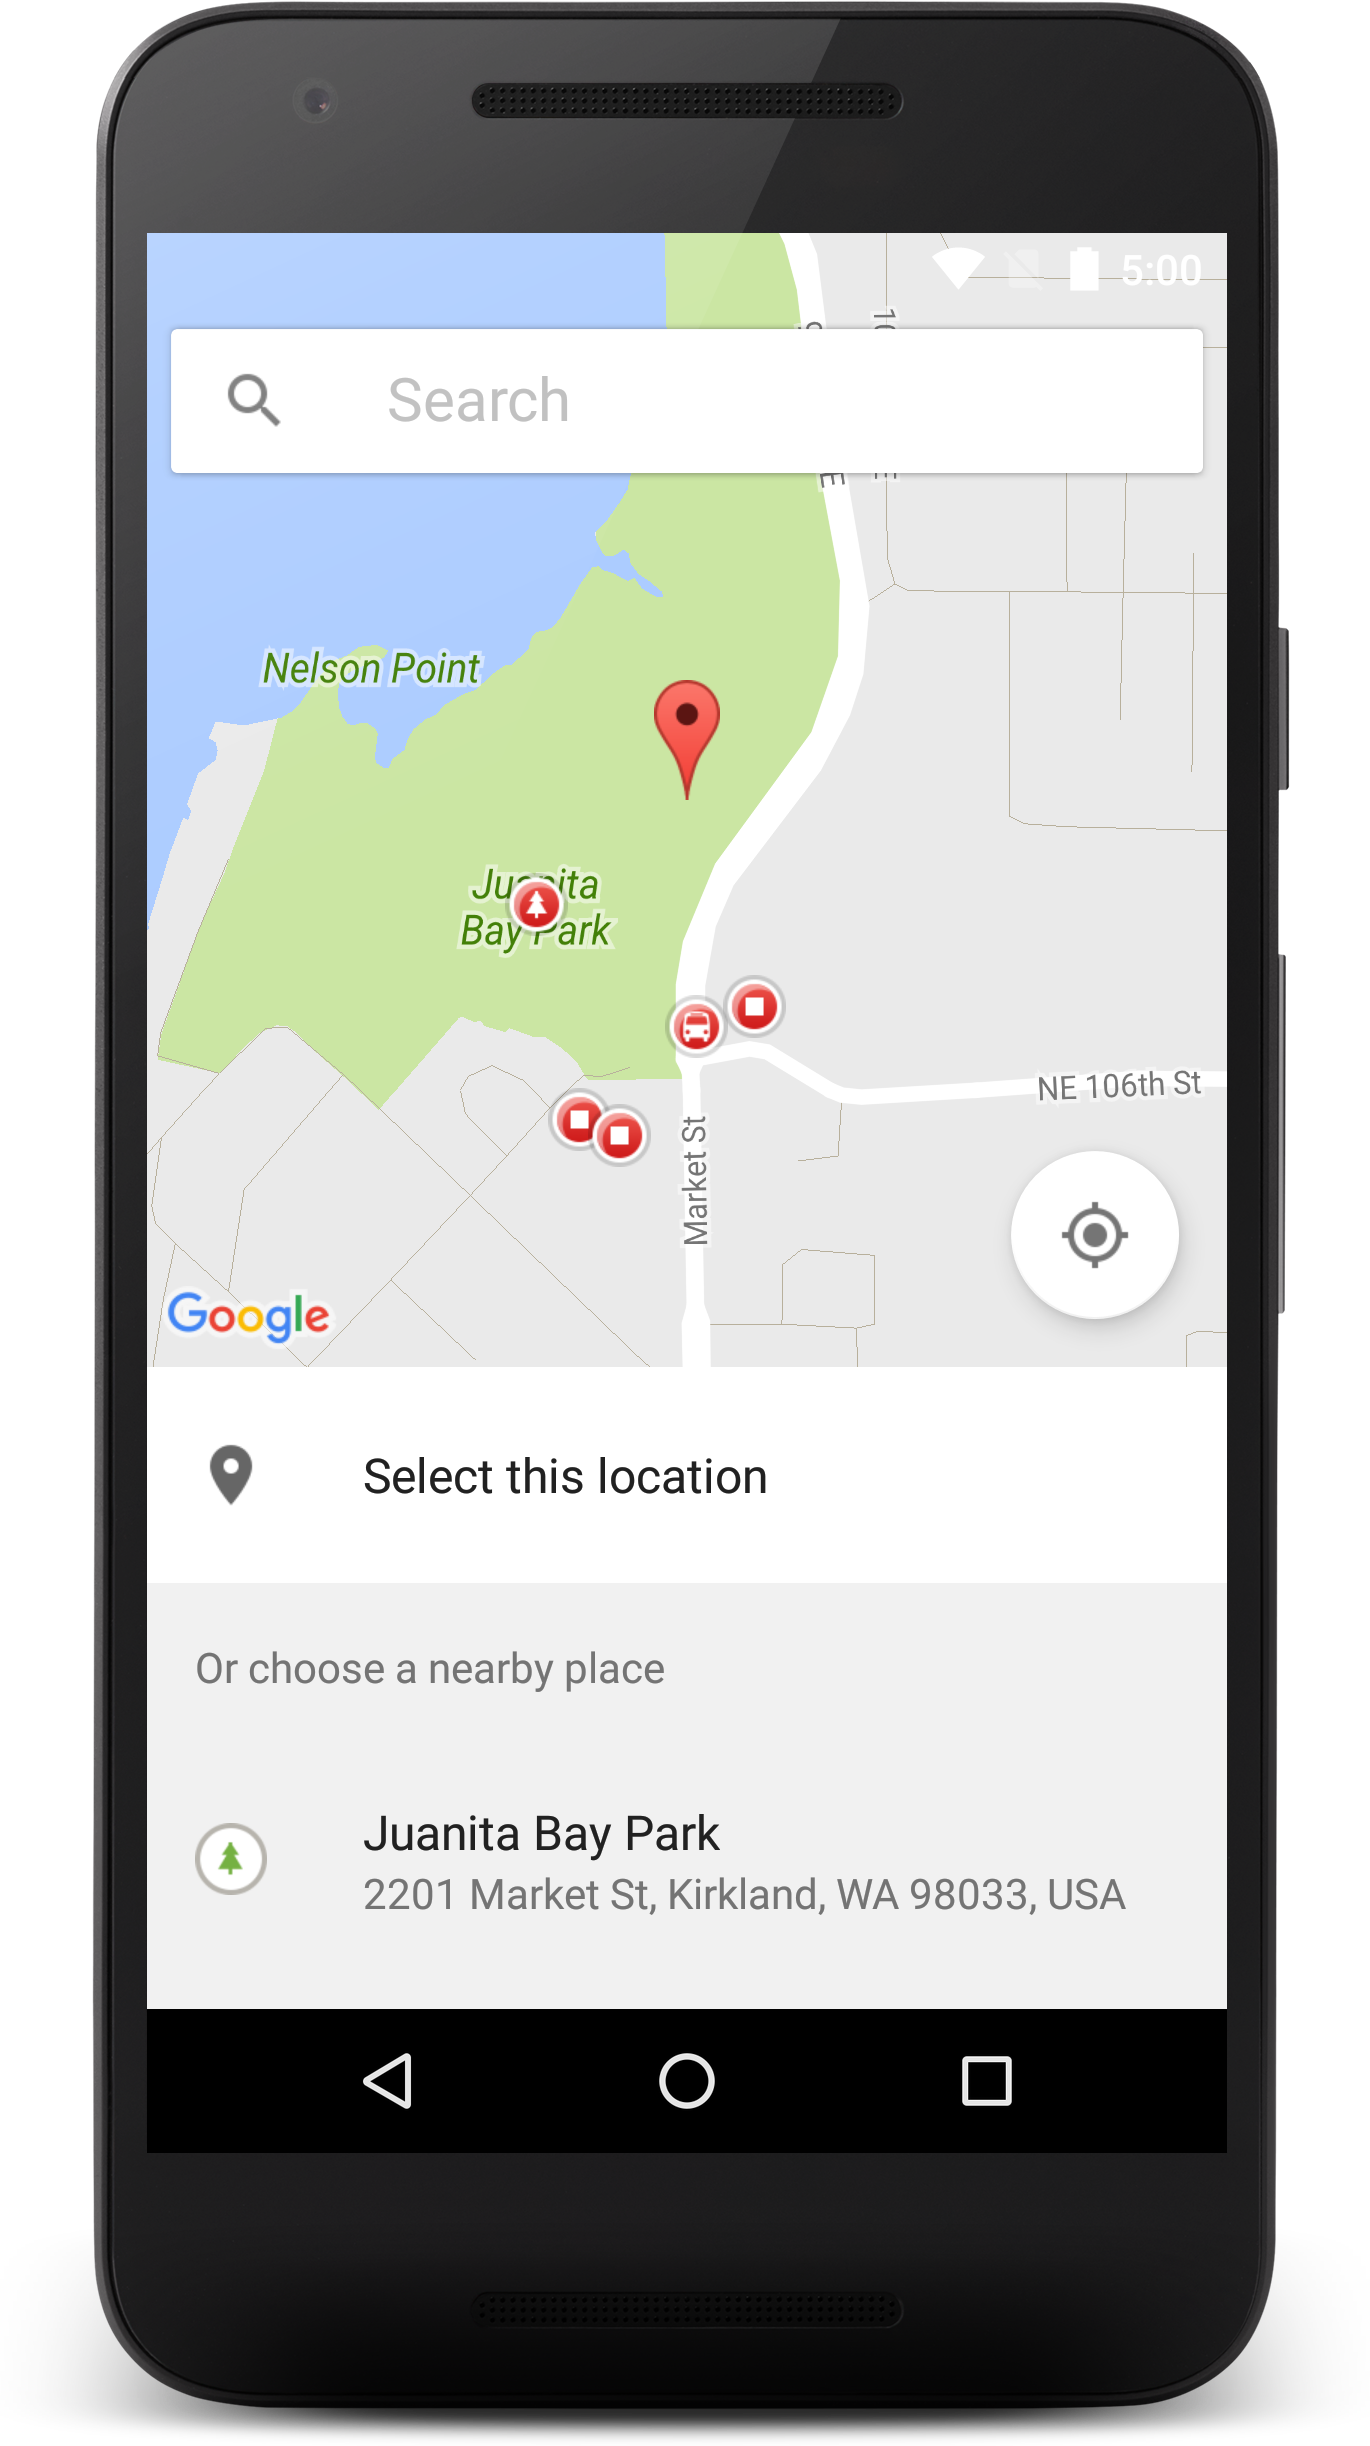
\includegraphics[height=.8\textheight]{location}
	\end{figure}
	\end{center}
\end{column}
\begin{column}{0.6\textwidth}
	acceptance criteria:
	\begin{itemize}
		\item search by current location 
		\item search by location name 
	\end{itemize}
\end{column}
\end{columns}
\end{frame}
\begin{frame}[fragile]
	How it looks like: simple state machine  (simplified) 
	\begin{figure}
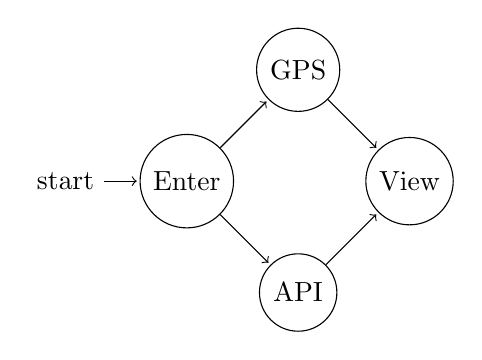
\begin{tikzpicture}[shorten >=1pt,node distance=2cm,on grid,auto] 
   \node[state,initial] (q_0)   {Enter}; 
   \node[state] (q_1) [above right=of q_0] {GPS}; 
   \node[state] (q_2) [below right=of q_0] {API}; 
   \node[state](q_3) [below right=of q_1] {View};
    \path[->] 
    (q_0) edge  node {} (q_1)
          edge  node [swap] {} (q_2)
    (q_1) edge  node  {} (q_3)
    (q_2) edge  node [swap] {} (q_3) ;
\end{tikzpicture}
	\end{figure}

\end{frame}
\begin{frame}[fragile]
\begin{columns}
\begin{column}{0.5\textwidth}
	\begin{center}
	\begin{figure}
		\centering
		
\includegraphics[height=.6\textheight]{tip}
	\end{figure}
	\end{center}
\end{column}
\begin{column}{0.6\textwidth}
	\begin{itemize}
		\item GPS connection is asynchronous and might fail
		\item Network requests are sent in parallel at each letter
		\item Debouncing 
		\item Latest takes priority (avoid overriding with old data) 
		\item Android lifecycle, etc
	\end{itemize}
\end{column}
\end{columns}

\end{frame}
\begin{frame}[fragile]
	``Concurrency is the composition of independently executing processes, typically functions, but they don't have to be.''
	``Parallelism is the simultaneous execution of multiple things, possibly related, possibly not.''

	Concurrency is a way to structure the computer programs. 
	Parallelism is \emph{not} the goal of concurrency

Rob Pike
\end{frame}
\begin{frame}[fragile]
Tony Horne seminal paper 
\end{frame}
\begin{frame}[fragile]
Java definition of concurrency and Leslie Lamport seminal paper 
\end{frame}
\begin{frame}[fragile]
Traditional picture of concurrency vs parallelism: coffe machine 
\end{frame}
\begin{frame}[fragile]
Better reppresentation: driving in the desert vs driving in London 
	\begin{figure}
		\centering
		\includegraphics{car-1}\\
		\includegraphics{car-2}
	\end{figure}
\end{frame}
\begin{frame}[fragile]
The deep problem: \emph{communication}

	Communicating, orchestrating independent processing. Software development as a \emph{dialog} between parts. 

	We will just sketch the surface of this deeper problem by focusing only  on a smaller technical problem in this talk: \emph{blocking} and \emph{non wasting unnecessary resources when waiting}
\end{frame}
\section{Blocking vs non-blocking}
\begin{frame}
	Test
%\begin{lstlisting}[language=Kotlin, basicstyle=\ttfamily]
%\end{lstlisting}
\end{frame}
\section{Demystifying coroutines}
\begin{frame}
What rae
\end{frame}
\section{Coroutines-powered concurrency models}
\begin{frame}[fragile]
\begin{itemize}
	\item CSP (aka, channels) 
\item actors 
	\end{itemize}
\end{frame}
\plain{Questions?}

%\begin{frame}[allowframebreaks] {References}
% \bibliography{demo}
% \bibliographystyle{abbrv}
%\end{frame}

\end{document}
\begin{lstlisting}[language=Kotlin, basicstyle=\ttfamily]
\end{lstlisting}
